\begin{figure}[htb]
\begin{centering}
{
	\begin{tikzpicture}[scale=0.75,place/.style={draw,circle,thick,text=white, text badly centered,minimum size=2.0in}]
		\node at (-2.5,-1.6) (M1) {\pgfbox[center,bottom]{\pgfuseimage{machine}}};
		\node at (2.5,-1.6) (M2) {\pgfbox[center,bottom]{\pgfuseimage{machine}}};
		\node at (0,2.9) (M3) {\pgfbox[center,bottom]{\pgfuseimage{machine}}};

		%\draw (0,0) circle (1cm);

		\draw (-4,-3) rectangle (-1.0,-1.5);
		\draw (1,-3) rectangle (4.0,-1.5);
		\draw (-1.5,1.5) rectangle (1.5,3);

		% Overall border
		\draw[draw=white] (-4.5,-3.5) rectangle (4.5,4.5);


		%\draw (-4.5,-3.5) rectangle (4.5,4.5);
		\filldraw[fill=blue,draw=black,opacity=0.2] (-3.8,-2.8) rectangle (-2.9,-1.6);
		\filldraw[gray, very thin,step=0.3cm,xshift=0.1cm,yshift=-0.1cm] (-3.9,-2.7) grid (-3.0,-1.5);
		\draw[black] (-3.8,-2.8) rectangle (-2.9,-1.6);

		\filldraw[fill=blue,draw=black,opacity=0.2] (-2.0,-2.8) rectangle (-1.1,-1.6);
		\filldraw[gray, very thin,step=0.3cm,xshift=0.1cm,yshift=-0.1cm] (-2.1,-2.7) grid (-1.2,-1.5);
		\draw[black] (-2.0,-2.8) rectangle (-1.1,-1.6);

		\node at (-1.45,-2.2) (S1) {$\mathcal{S}^{(2)}_1$};
		\node at (-3.3,-2.2) {$\mathcal{S}^{(1)}_1$};


		\filldraw[fill=red,draw=black,opacity=0.2] (3.8,-2.8) rectangle (2.9,-1.6);
		\filldraw[gray, very thin,step=0.3cm,xshift=-0.1cm,yshift=-0.1cm] (3.0,-2.7) grid (3.9,-1.5);
		\draw[black] (3.8,-2.8) rectangle (2.9,-1.6);

		\filldraw[fill=red,draw=black,opacity=0.2] (2.0,-2.8) rectangle (1.1,-1.6);
		\filldraw[gray, very thin,step=0.3cm,xshift=-0.1cm,yshift=-0.1cm] (1.2,-2.7) grid (2.1,-1.5);
		\draw[black] (2.0,-2.8) rectangle (1.1,-1.6);

		\node at (1.6,-2.2) {$\mathcal{S}^{(1)}_2$};
		\node at (3.4,-2.2) (S2) {$\mathcal{S}^{(2)}_2$};


		\filldraw[fill=green,draw=black,opacity=0.2] (-1.3,1.7) rectangle (-0.4,2.9);
		\filldraw[gray, very thin,step=0.3cm,xshift=0.2cm,yshift=0.2cm] (-1.5,1.5) grid (-0.6,2.7);
		\draw[black] (-1.3,1.7) rectangle (-0.4,2.9);

		\filldraw[fill=green,draw=black,opacity=0.2] (1.3,1.7) rectangle (0.4,2.9);
		\filldraw[gray, very thin,step=0.3cm,xshift=-0.2cm,yshift=0.2cm] (0.6,1.5) grid (1.5,2.7);
		\draw[black] (1.3,1.7) rectangle (0.4,2.9);

		\node at (-0.8,2.35) {$\mathcal{S}^{(1)}_3$};
		\node at  (0.9,2.35) (S3) {$\mathcal{S}^{(2)}_3$};
		%\node at (3.4,-2.2) {$\mathcal{S}^{(2)}_2$};


		\begin{scope}[>=stealth,ultra thick,->]
		\path (S1) edge[bend right=30]  node [left=5pt] { } (S2);
		\path (S2) edge[bend right=30]  node [left=5pt] { } (S3);
		\path (S3) edge[bend right=30]  node [left=5pt] { } (S1);

		%\path (S) edge[red,bend right=10,decorate,decoration={snake,amplitude=1mm}] 
			%node [right=5pt,text=black] {$\beta_1$ } (I1);
		%\path (I1) edge[red,bend right=10,decorate,decoration={snake,amplitude=1mm}] 
			%node [right=5pt,text=black] {$\epsilon \beta_2$ } (I12);

		%\path (I12) edge[bend right=20]     node [left=5pt] {$\delta_2$} (I1);
		
			%\path (S) edge[red,bend left=10,decorate,decoration={snake,amplitude=1mm}] 
				%node [left=5pt,text=black] {$\beta_2$ } (I2);
			%\path (I2) edge[bend left=20]     node [right=5pt] {$\delta_2$} (S);

			%\path (I2) edge[red,bend left=10,decorate,decoration={snake,amplitude=1mm}] 
				%node [left=5pt,text=black] {$\epsilon \beta_1$ } (I12);
			%\path (I12) edge[bend left=20]     node [right=5pt] {$\delta_1$} (I2);


		\end{scope}
	\end{tikzpicture}
}
\caption{Movement of parameters through the cloud between subepochs.
\label{fig:data-movement}
}
\end{centering}
\end{figure}



%%%%% GENEREAL GRID
%\begin{figure}[htb]
%\begin{centering}
%{
	%\begin{tikzpicture}[scale=1.00,place/.style={draw,circle,thick,text=white, text badly centered,minimum size=2.0in}]

		%\filldraw[gray, very thin,step=0.2cm,yshift=0.1cm] (-2.2,2) grid (2,3);
		%\filldraw[gray, very thin,step=0.2cm,xshift=-0.1cm] (-3.2,-2.2) grid (-2.2,2);

		%\filldraw[gray, very thin,step=0.2cm] (-2.2,-2.2) grid (2,2);


		%\draw[black] (-2.2,-2.2) rectangle (2,2);
		%\draw[black] (-3.3,-2.2) rectangle (-2.3,2);
		%\draw[black] (-2.2,2.1) rectangle (2,3.1);


		%\draw[black] (-0.8,-2.2) rectangle (0.6,2);
		%\draw[black] (-2.2,-0.8) rectangle (2.0,0.6);

		%\draw[black] (-3.3,-0.8) rectangle (-2.3,0.6);
		%\draw[black] (-0.8,2.1) rectangle (0.6,3.1);

	%\end{tikzpicture}
%}
%\caption{tikz grid breakdown
%\label{fig:data-movement}
%}
%\end{centering}
%\end{figure}

\definecolor{lightgray}{gray}{0.85}
\def\colorOpacity{0.4}
\def\gridScaling{0.78}
\begin{figure*}
	\centering{
	\begin{minipage}{0.24\textwidth}
		\centering {
		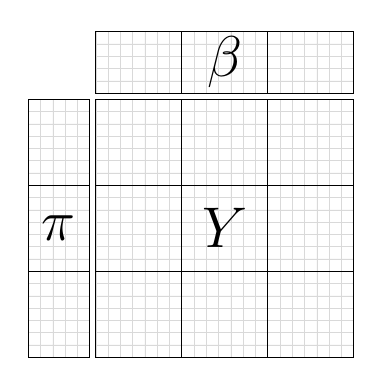
\begin{tikzpicture}[scale=\gridScaling,place/.style={draw,circle,thick,text=white, text badly centered,minimum size=2in}]

			\filldraw[lightgray, very thin,step=0.2cm,yshift=0.1cm] (-2.2,2) grid (2,3);
			\filldraw[lightgray, very thin,step=0.2cm,xshift=-0.1cm] (-3.2,-2.2) grid (-2.2,2);
			\filldraw[lightgray, very thin,step=0.2cm] (-2.2,-2.2) grid (2,2);


			\draw[black] (-2.2,-2.2) rectangle (2,2);
			\draw[black] (-3.3,-2.2) rectangle (-2.3,2);
			\draw[black] (-2.2,2.1) rectangle (2,3.1);


			\draw[black] (-0.8,-2.2) rectangle (0.6,2);
			\draw[black] (-2.2,-0.8) rectangle (2.0,0.6);

			\draw[black] (-3.3,-0.8) rectangle (-2.3,0.6);
			\draw[black] (-0.8,2.1) rectangle (0.6,3.1);

			\tikzstyle{every node}=[font=\huge]
			\node at (-0.1,-0.1) {$Y$};
			\node at (-2.8,-0.1) {$\pi$};
			\node at (-0.1,2.6) {$\beta$};
		\end{tikzpicture}
		}
	\end{minipage}
	\begin{minipage}{0.24\textwidth}
		\centering {
		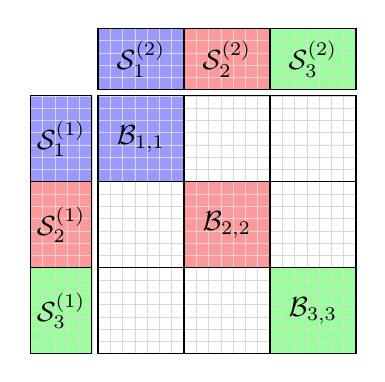
\begin{tikzpicture}[scale=\gridScaling,place/.style={draw,circle,thick,text=white, text badly centered,minimum size=2in}]


			\filldraw[fill=green,draw=black,opacity=\colorOpacity] (-3.3,-2.2) rectangle (-2.3,-0.8);
			\filldraw[fill=red,draw=black,opacity=\colorOpacity] (-3.3,-0.8) rectangle (-2.3,0.6);
			\filldraw[fill=blue,draw=black,opacity=\colorOpacity] (-3.3,0.6) rectangle (-2.3,2);

			\filldraw[fill=blue,draw=black,opacity=\colorOpacity] (-2.2,2.1) rectangle (-0.8,3.1);
			\filldraw[fill=red,draw=black,opacity=\colorOpacity] (-0.8,2.1) rectangle (0.6,3.1);
			\filldraw[fill=green,draw=black,opacity=\colorOpacity] (0.6,2.1) rectangle (2,3.1);

			\filldraw[fill=blue,draw=black,opacity=\colorOpacity] (-2.2,0.6) rectangle (-0.8,2);
			\filldraw[fill=red,draw=black,opacity=\colorOpacity] (-0.8,-0.8) rectangle (0.6,0.6);
			\filldraw[fill=green,draw=black,opacity=\colorOpacity] (0.6,-2.2) rectangle (2,-0.8);


			\filldraw[lightgray, very thin,step=0.2cm,yshift=0.1cm] (-2.2,2) grid (2,3);
			\filldraw[lightgray, very thin,step=0.2cm,xshift=-0.1cm] (-3.2,-2.2) grid (-2.2,2);
			\filldraw[lightgray, very thin,step=0.2cm] (-2.2,-2.2) grid (2,2);


			\draw[black] (-2.2,-2.2) rectangle (2,2);
			\draw[black] (-3.3,-2.2) rectangle (-2.3,2);
			\draw[black] (-2.2,2.1) rectangle (2,3.1);


			\draw[black] (-0.8,-2.2) rectangle (0.6,2);
			\draw[black] (-2.2,-0.8) rectangle (2.0,0.6);

			\draw[black] (-3.3,-0.8) rectangle (-2.3,0.6);
			\draw[black] (-0.8,2.1) rectangle (0.6,3.1);

			\tikzstyle{every node}=[font=\normalsize]
			\node at (-1.5,1.3) {$\mathcal{B}_{1,1}$};
			\node at (-0.1,-0.1) {$\mathcal{B}_{2,2}$};
			\node at (1.3,-1.5) {$\mathcal{B}_{3,3}$};

			\node at (-2.8,1.3) {$\mathcal{S}_1^{(1)}$};
			\node at (-2.8,-0.1) {$\mathcal{S}_2^{(1)}$};
			\node at (-2.8,-1.5) {$\mathcal{S}_3^{(1)}$};

			\node at (1.3,2.6) {$\mathcal{S}_3^{(2)}$};
			\node at (-0.1,2.6) {$\mathcal{S}_2^{(2)}$};
			\node at (-1.5,2.6) {$\mathcal{S}_1^{(2)}$};

		\end{tikzpicture}
		}
	\end{minipage}
	\begin{minipage}{0.24\textwidth}
		\centering {
		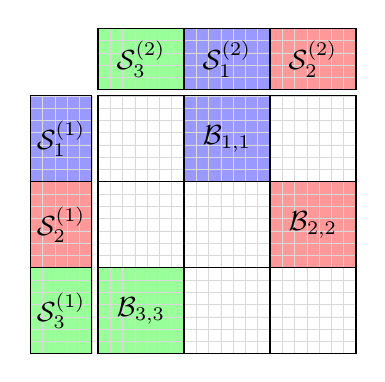
\begin{tikzpicture}[scale=\gridScaling,place/.style={draw,circle,thick,text=white, text badly centered,minimum size=2in}]


			\filldraw[fill=green,draw=black,opacity=\colorOpacity] (-3.3,-2.2) rectangle (-2.3,-0.8);
			\filldraw[fill=red,draw=black,opacity=\colorOpacity] (-3.3,-0.8) rectangle (-2.3,0.6);
			\filldraw[fill=blue,draw=black,opacity=\colorOpacity] (-3.3,0.6) rectangle (-2.3,2);

			\filldraw[fill=green,draw=black,opacity=\colorOpacity] (-2.2,2.1) rectangle (-0.8,3.1);
			\filldraw[fill=blue,draw=black,opacity=\colorOpacity] (-0.8,2.1) rectangle (0.6,3.1);
			\filldraw[fill=red,draw=black,opacity=\colorOpacity] (0.6,2.1) rectangle (2,3.1);

			\filldraw[fill=blue,draw=black,opacity=\colorOpacity] (-0.8,0.6) rectangle (0.6,2);
			\filldraw[fill=red,draw=black,opacity=\colorOpacity] (0.6,-0.8) rectangle (2.0,0.6);
			\filldraw[fill=green,draw=black,opacity=\colorOpacity] (-2.2,-2.2) rectangle (-0.8,-0.8);


			\filldraw[lightgray, very thin,step=0.2cm,yshift=0.1cm] (-2.2,2) grid (2,3);
			\filldraw[lightgray, very thin,step=0.2cm,xshift=-0.1cm] (-3.2,-2.2) grid (-2.2,2);
			\filldraw[lightgray, very thin,step=0.2cm] (-2.2,-2.2) grid (2,2);


			\draw[black] (-2.2,-2.2) rectangle (2,2);
			\draw[black] (-3.3,-2.2) rectangle (-2.3,2);
			\draw[black] (-2.2,2.1) rectangle (2,3.1);


			\draw[black] (-0.8,-2.2) rectangle (0.6,2);
			\draw[black] (-2.2,-0.8) rectangle (2.0,0.6);

			\draw[black] (-3.3,-0.8) rectangle (-2.3,0.6);
			\draw[black] (-0.8,2.1) rectangle (0.6,3.1);

			\tikzstyle{every node}=[font=\normalsize]
			\node at (-0.1,1.3) {$\mathcal{B}_{1,1}$};
			\node at (1.3,-0.1) {$\mathcal{B}_{2,2}$};
			\node at (-1.5,-1.5) {$\mathcal{B}_{3,3}$};

			\node at (-2.8,1.3) {$\mathcal{S}_1^{(1)}$};
			\node at (-2.8,-0.1) {$\mathcal{S}_2^{(1)}$};
			\node at (-2.8,-1.5) {$\mathcal{S}_3^{(1)}$};

			\node at (1.3,2.6) {$\mathcal{S}_2^{(2)}$};
			\node at (-0.1,2.6) {$\mathcal{S}_1^{(2)}$};
			\node at (-1.5,2.6) {$\mathcal{S}_3^{(2)}$};

		\end{tikzpicture}
		}
	\end{minipage}
	\begin{minipage}{0.24\textwidth}
		\centering {
		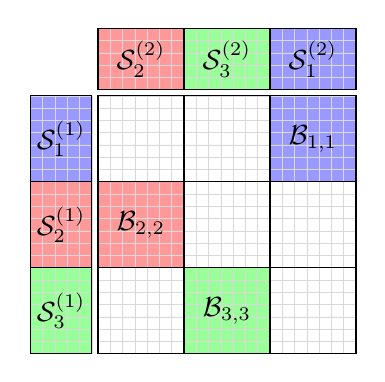
\begin{tikzpicture}[scale=\gridScaling,place/.style={draw,circle,thick,text=white, text badly centered,minimum size=2in}]


			\filldraw[fill=green,draw=black,opacity=\colorOpacity] (-3.3,-2.2) rectangle (-2.3,-0.8);
			\filldraw[fill=red,draw=black,opacity=\colorOpacity] (-3.3,-0.8) rectangle (-2.3,0.6);
			\filldraw[fill=blue,draw=black,opacity=\colorOpacity] (-3.3,0.6) rectangle (-2.3,2);

			\filldraw[fill=red,draw=black,opacity=\colorOpacity] (-2.2,2.1) rectangle (-0.8,3.1);
			\filldraw[fill=green,draw=black,opacity=\colorOpacity] (-0.8,2.1) rectangle (0.6,3.1);
			\filldraw[fill=blue,draw=black,opacity=\colorOpacity] (0.6,2.1) rectangle (2,3.1);

			\filldraw[fill=blue,draw=black,opacity=\colorOpacity] (0.6,0.6) rectangle (2.0,2);
			\filldraw[fill=red,draw=black,opacity=\colorOpacity] (-2.2,-0.8) rectangle (-0.8,0.6);
			\filldraw[fill=green,draw=black,opacity=\colorOpacity] (-0.8,-2.2) rectangle (0.6,-0.8);


			\filldraw[lightgray, very thin,step=0.2cm,yshift=0.1cm] (-2.2,2) grid (2,3);
			\filldraw[lightgray, very thin,step=0.2cm,xshift=-0.1cm] (-3.2,-2.2) grid (-2.2,2);
			\filldraw[lightgray, very thin,step=0.2cm] (-2.2,-2.2) grid (2,2);


			\draw[black] (-2.2,-2.2) rectangle (2,2);
			\draw[black] (-3.3,-2.2) rectangle (-2.3,2);
			\draw[black] (-2.2,2.1) rectangle (2,3.1);


			\draw[black] (-0.8,-2.2) rectangle (0.6,2);
			\draw[black] (-2.2,-0.8) rectangle (2.0,0.6);

			\draw[black] (-3.3,-0.8) rectangle (-2.3,0.6);
			\draw[black] (-0.8,2.1) rectangle (0.6,3.1);

			\tikzstyle{every node}=[font=\normalsize]
			\node at (1.3,1.3) {$\mathcal{B}_{1,1}$};
			\node at (-1.5,-0.1) {$\mathcal{B}_{2,2}$};
			\node at (-0.1,-1.5) {$\mathcal{B}_{3,3}$};

			\node at (-2.8,1.3) {$\mathcal{S}_1^{(1)}$};
			\node at (-2.8,-0.1) {$\mathcal{S}_2^{(1)}$};
			\node at (-2.8,-1.5) {$\mathcal{S}_3^{(1)}$};

			\node at (1.3,2.6) {$\mathcal{S}_1^{(2)}$};
			\node at (-0.1,2.6) {$\mathcal{S}_3^{(2)}$};
			\node at (-1.5,2.6) {$\mathcal{S}_2^{(2)}$};

		\end{tikzpicture}
		}
	\end{minipage}
	
	%$\quad\quad\quad$
	%\begin{minipage}{0.25\textwidth}
		%\centering{\includegraphics[page=9,width=0.95\linewidth]{figs/figures.pdf}\\(b)}
	%\end{minipage}
	%$\quad\quad\quad$
	%\begin{minipage}{0.25\textwidth}
		%\centering{\includegraphics[page=7,width=0.95\linewidth]{figs/figures.pdf}\\(c)
		%}
	%\end{minipage}
	}
\label{fig:batched}
\end{figure*}





%\begin{figure}[htb]
%\begin{centering}
%{
	%\begin{tikzpicture}[scale=1,place/.style={draw,circle,thick,text=white, text badly centered,minimum size=0.3in}]
		%%\node[fill=blue!65,place] at (0, -2.5) (S) {\textbf{S}};
		%\node[place] at (0,-2.5) (S) {\pgfbox[center,bottom]{\pgfuseimage{machine}}};
		%\node[fill=gray,place]  at (-2.5, 0)  (I1) {$\mathbf{I_1}$}; 
		%\node[fill=gray, place]   at (2.5, 0)  (I2) {$\mathbf{I_2}$};
		%\node[fill=black, place]   at (0, 2.5)  (I12) {$\mathbf{I_{1,2}}$};
			%%\node[place] at (1, 0) (E) {\textbf{E}};
		%%\node[place] at (2, -0.5) (I) {\textbf{I}};	
		%%\node[place] at (0,-1.5) (V) {\textbf{V}};
		%\begin{scope}[>=stealth,ultra thick,->]

		%\path (S) edge[red,bend right=10,decorate,decoration={snake,amplitude=1mm}] 
			%node [right=5pt,text=black] {$\beta_1$ } (I1);
		%\path (I1) edge[bend right=20]     node [left=5pt] {$\delta_1$} (S);
		%\path (I1) edge[red,bend right=10,decorate,decoration={snake,amplitude=1mm}] 
			%node [right=5pt,text=black] {$\epsilon \beta_2$ } (I12);

		%\path (I12) edge[bend right=20]     node [left=5pt] {$\delta_2$} (I1);
		
			%\path (S) edge[red,bend left=10,decorate,decoration={snake,amplitude=1mm}] 
				%node [left=5pt,text=black] {$\beta_2$ } (I2);
			%\path (I2) edge[bend left=20]     node [right=5pt] {$\delta_2$} (S);

			%\path (I2) edge[red,bend left=10,decorate,decoration={snake,amplitude=1mm}] 
				%node [left=5pt,text=black] {$\epsilon \beta_1$ } (I12);
			%\path (I12) edge[bend left=20]     node [right=5pt] {$\delta_1$} (I2);


		%\end{scope}
	%\end{tikzpicture}
%}
%\caption{State Diagram for a node in the graph under our partial-competition model.
%% $SI_1I_2S$ competing viruses model. The node is in the $S$ state if it doesn't have either  competitor (say iPhone or Android). It is in $I_1$ if it gets the iPhone (virus 1) and is in $I_2$ if it gets the Android (virus 2). The transitions from $S$ to $I_1$ or $I_2$ (red-curvy arrows) depend on the infected neighbors of the node. The remaining transitions,  in contrast, are self-transitions, without the aid of any neighbor.
%\label{fig:siismodel}
%}
%\end{centering}
%\end{figure}



%\begin{tikzpicture}[scale=1.5]
    %% Draw axes
    %\draw [<->,thick] (0,2) node (yaxis) [above] {$y$}
        %|- (3,0) node (xaxis) [right] {$x$};
    %% Draw two intersecting lines
    %\draw (0,0) coordinate (a_1) -- (2,1.8) coordinate (a_2);
    %\draw (0,1.5) coordinate (b_1) -- (2.5,0) coordinate (b_2);
    %% Calculate the intersection of the lines a_1 -- a_2 and b_1 -- b_2
    %% and store the coordinate in c.
    %\coordinate (c) at (intersection of a_1--a_2 and b_1--b_2);
    %% Draw lines indicating intersection with y and x axis. Here we use
    %% the perpendicular coordinate system
    %\draw[dashed] (yaxis |- c) node[left] {$y'$}
        %-| (xaxis -| c) node[below] {$x'$};
    %% Draw a dot to indicate intersection point
    %\fill[red] (c) circle (2pt);
	%%\pgfuseimage{machine}
%\end{tikzpicture}


\begin{figure*}
	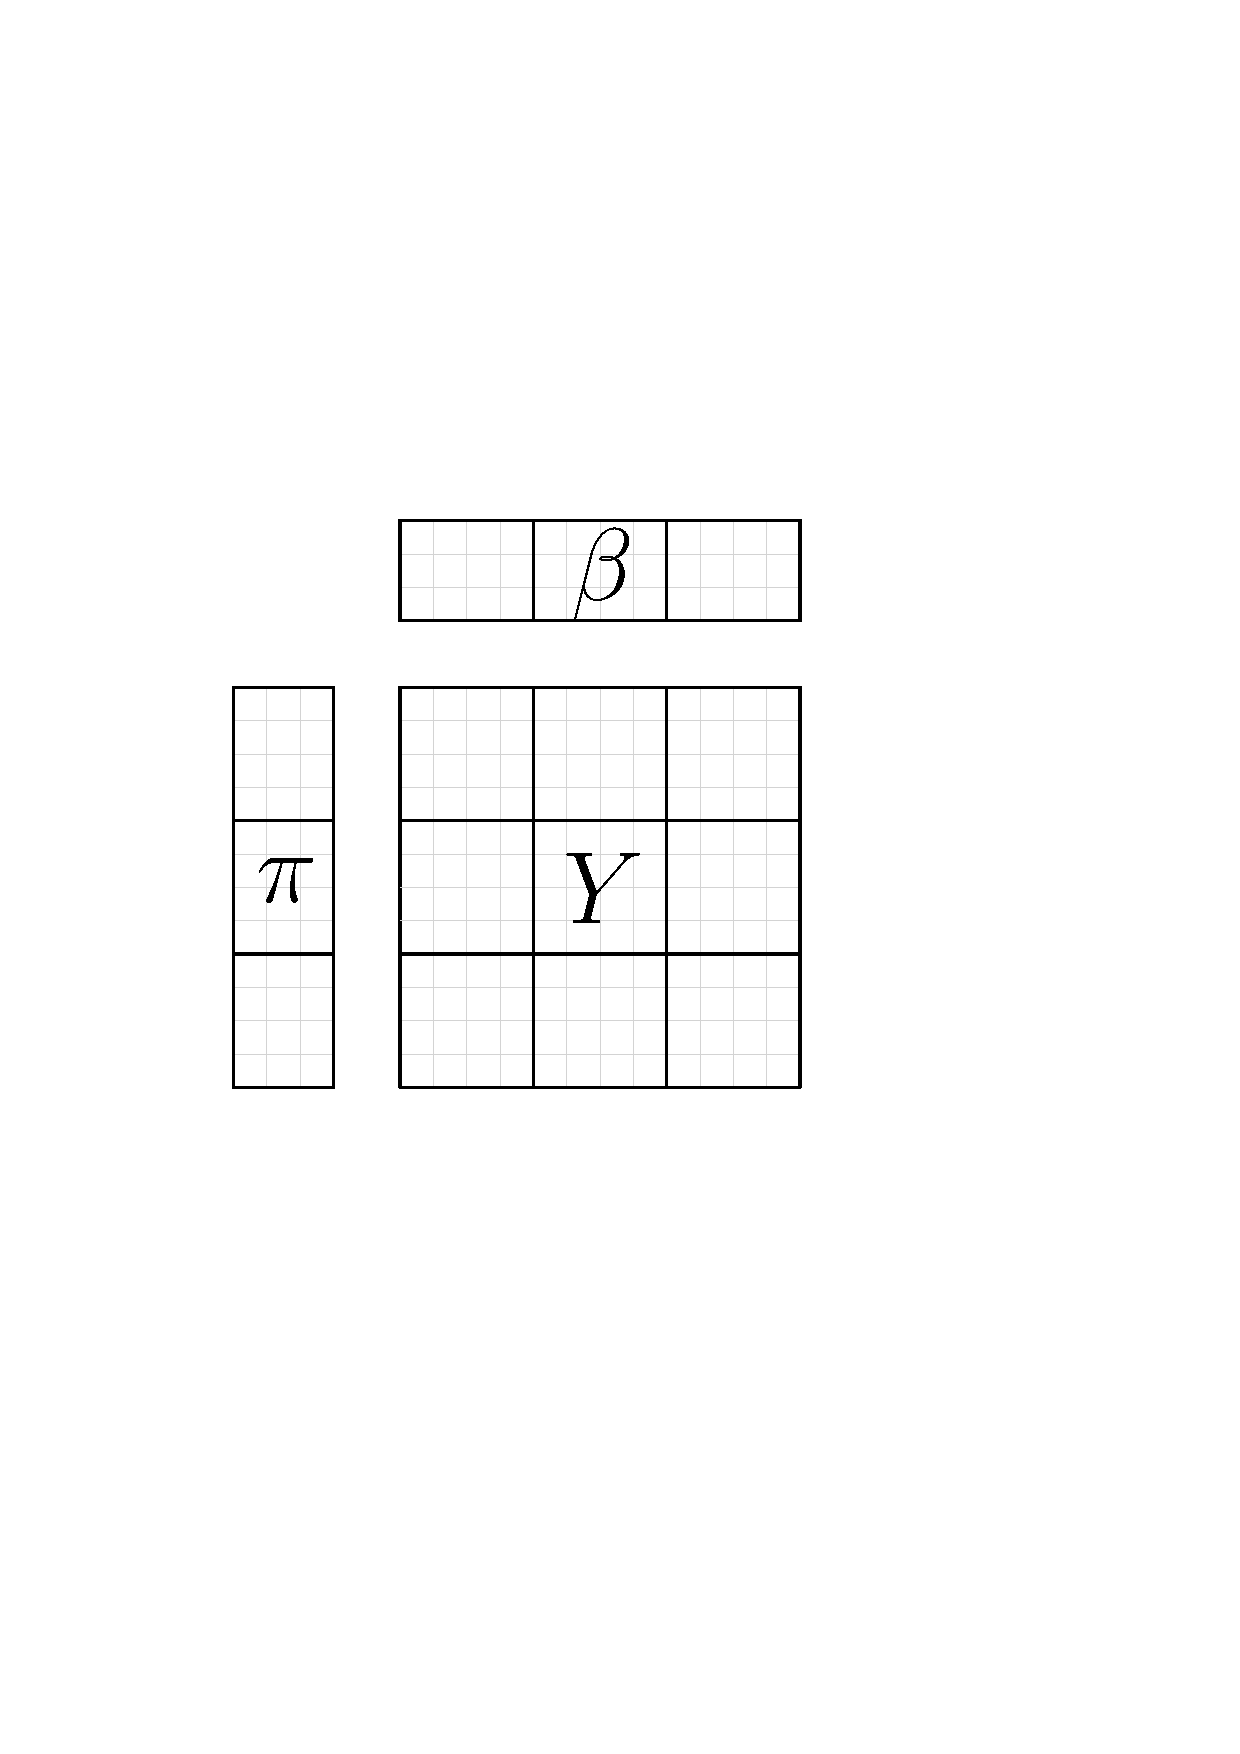
\includegraphics[page=1, width=0.24\textwidth]{figs/grid3.pdf} \hfill
	\includegraphics[page=2, width=0.24\textwidth]{figs/grid3.pdf} \hfill
	\includegraphics[page=13,width=0.24\textwidth]{figs/grid3.pdf} \hfill
	\includegraphics[page=17,width=0.24\textwidth]{figs/grid3.pdf} 
	\caption{Example of data and model partitioning along with the three subepochs.}
	\label{fig:partition}
\end{figure*}

In designing any large scale machine learning system, one of the most important
design decisions is the abstraction for the data and problem model.  Recent
distributed ML systems focus primarily on the abstraction for the data, such as
\graphlab's \cite{Low:DGF} view of each data point as a node or 
\psgd's \cite{zinkevich2010parallelized} view of partitioning only on the data.
Here we take a different approach - partitioning our data and the model we are building of the
data simultaneously.  As we will go on to demonstrate, focusing on both is
advantageous for both scalability and speed.

\subsection{Block structure in relational data} % (fold)
\label{sub:Block structure in relational data}

For many classic machine learning problems, we have relational data between
two sets of entities, and we are asking questions about these entities. \abhi{my editing is here} 
Answers to 
these questions are obtained by estimating a set of unknown that define the relations
concretely. These unknowns can be categorized into two sets: 1) variables ($V$) and 2) parameters ($P$). 
Variables are set of unknowns that arise due to the data and are dependent on dataset characteristics.
Parameters are set of unknowns that arise due to the assumptions that one makes in the entity relationship
(i.e. the model).
The overall unknowns set (variable and parameters) can be divided into relational blocks ($b$) of independent set of 
unknowns($\gamma_b$) for most problems. The number of these unknown() depend on the data size well as the parameteric 
assumptions of the relationship (i.e. the model we are estimating). 
To be a
bit more concrete, consider the classic topic modeling question: given a large set
of $D$ documents, with what probability a given document talks about a given
topic, and with what probability does a given topic has a given word~\cite{Blei:2003:LDA}? 
In this case, a raw data point is the number of occurrences of a word in a
document. Each data point is an element in the document by word data matrix. We
normalize the data matrix to obtain matrix $Y$ where an element
$Y_{i,j}$ in column $i$ and row $j$ in the new matrix is the original
element at $(i,j)$ divided by the row $i$'s sum. In simple terms,
$Y_{i,j} = p(j|i)$ i.e. the probability of word $j$ lying in
document $i$.

\lda (topic modelling) assumes that there are fixed number ($K$) of
underlying topics in the document corpus. A topic is composed of weighted
combinations of words in the corpus where different words have different
weights. The weight of a word $j$ in topic $k$  is $p(j|k)$: probability of
word $j$ in topic $k$. Each document in the corpus is a weighted combination of
the topics. The weight of topic $k$ in document $i$ is $p(k|i)$. The probability
of a word $i$ in document $j$ is 
\begin{equation}
p(j|i)=\sum_{k=1}^Kp(j|k)*p(k|i)
\end{equation}

We define two matrices $\pi$ and $\beta$ such that $\pi_{i,k}=p(k|i)$ and
$\beta_{k,j}=p(j|k)$. In that case $Y_{i,j}=\sum_k\pi_{i,k}*\beta_{k,j}$.
The $\pi$ matrix is the per document topic probability matrix. $\pi_{i,k}$ is
the probability weight of topic $k$ in document $j$. $\beta$ matrix is the per
topic word probability. $\beta_{k,j}$ is the probability weight of word $j$
in topic $k$. In \lda we are solving the following query to find $\pi$ and
$\beta$.

% {\small
\begin{align}
&\argmin_{\pi,\beta}L(Y,\pi,\beta)
=\sum_{i,j}(Y_{i,j}-\sum_k\pi_{i,k}\beta_{k,j})^2
%= \sum_{i,j}(Y_{i,j}-\sum_k \pi_{i,k}\beta_{k,j})_p^p
\label{eqn:LDA}\\
&\text{s.t.} \; \forall  i,j,k \quad
\sum_k\pi_{i,k}=1,
\sum_j\beta_{k,j}=1, \quad
\pi_{i,k}\geq 0,
\beta_{k,j}\geq 0,
\nonumber
\end{align}
% }

The second line of constraints in equation~\ref{eqn:LDA} is due to the fact that
$\pi$ and $\beta$ are probability matrices. 

Because of the intrinsic relational nature of the data (here between words and
documents), partitioning our data ($Y$) intelligently results in a clean
partitioning of our model of topics for the words and documents.

More specifically, for any given subset of the documents and subset of the
words, there is a unique set of data points that are applicable to entities from
both sets.  If we view our data as a very sparse matrix $Y$ (where $Y$ is a
documents by word matrix), partitioning the documents and the words results in
the data matrix $Y$ also being partitioned into blocks, as seen in Figure
\ref{fig:abstraction}.
Under this partitioning, all data points in block $\mathcal{B}_{i,j}$ describe
a relationship between a word from set $\mathcal{S}^{(1)}_i$ and document from
set $\mathcal{S}^{(2)}_j$.  We focus our computation around these blocks of data.

An interesting property of these blocks is that for some blocks, such as
$\mathcal{B}_{i,j}$ and $\mathcal{B}_{i',j'}$ where $i\neq i'$ and $j \neq j'$,
we see that the blocks are \textit{independent}.  That is, a data point from
$\mathcal{B}_{i,j}$ does not describe any relations to words in
$\mathcal{S}^{(1)}_{i'}$ or documents in $\mathcal{S}^{(2)}_{j'}$ and vice
versa for data in $\mathcal{B}_{i',j'}$.
%Formally defined:
%\alex{add formal definition of independence here? or will that come off too
%mathy}
As has been shown in previous stochastic learning literature \cite{textbook}
and used in simpler data mining problems \cite{gemulla,flexifact}, this
independence property allows for improved scalability and parallel processing.
We will discuss our system and the strengths of this abstraction primarily in
terms of topic modeling,
%Note, we will primarily discuss
%this system in terms of topic modeling, 
but note the system generalizes to many
machine learning problems as we will demonstrate later.
%We go over the implications for topic modeling and other machine learning
%problems below.

\subsection{Distributing our data} % (fold)
\label{sub:Distributing the Data and Model}

As mentioned above, distributing your data over a cluster is useful, but as
data grows partitioning both the data and your model of that data is
increasingly valuable.  For example, if we would like to know the topic
distribution for 10 million documents over 1000 topics, this would require over
37 gigabytes just to hold all of the answers to the query.  Therefore, it is
crucial that as our data grows we intelligently distribute both the data and our
solution.  This significantly improve memory efficiency and makes it possible
to scale to unprecedented sizes.  Luckily, our blocking abstraction makes this
easy.

In processing a given block $\mathcal{B}_{i,j}$, we only need the data from
that block, and the current information about the words $\mathcal{S}^{(1)}_{i}$
and documents $\mathcal{S}^{(2)}_{j}$.  Therefore, in distributing the problem
over a cluster of machines, we can have each worker only store and process one
block and its corresponding object model at a time.  Additionally, because our
sets of documents and sets of words are each disjoint, we can process our
blocks in such a way that each document and each word is only being worked on
by one worker at a time.  As a result, we do not need to store \textit{any}
duplicate data (about the topic model or blocks) and thus we are perfectly
memory efficient.


% subsection Distributing the Data and Model (end)

\subsection{Parallel processing} % (fold)
The last piece of the general system design is understanding the order in which
we process our data.  Our goal is to reach the optimal memory efficiency
described above and also keep our computation fast and accurate.  To do this,
we must choose a \textit{stratum}, a group of blocks, to process in parallel.  
In order to be memory efficient and keep our computation accurate, each stratum
must only contain blocks that are independent of each other.  From the block
structure, we can create multiple strata such that each block is in exactly one
stratum.
We iterate over the strata, in each case processing each block
in the stratum in parallel on the cluster.  We call processing one stratum a
\textit{subepoch} and processing all of the strata an \textit{epoch}.
A small example can be seen in Figure \ref{fig:abstraction}.

In practice, each machine in the cluster holds one of the blocks being
currently processed as well as the topic model for the corresponding words and
documents. As explained, doing this results in the topic models and blocks
being stored exactly once and thus being memory efficient.  
%We call the processing of all of the data from all of the blocks in a given stratum a \textit{subepoch}.
When a subepoch completes, we load the blocks for the next subepoch and
transfer the necessary pieces of the topic model to the appropriate machines.
\alex{maybe give classic systems graphic of data moving between machines in
cluster?}


% subsection Processing the data (end)



%\subsection{Topic Modelling} \abhi{explain the model and data partition using
%this, topic-word and doc-topic matrix}
